	\documentclass[10pt,oneside]{CBFT_book}
	% Algunos paquetes
	\usepackage{amssymb}
	\usepackage{amsmath}
	\usepackage{graphicx}
% 	\usepackage{libertine}
% 	\usepackage[bold-style=TeX]{unicode-math}
	\usepackage{lipsum}

	\usepackage{natbib}
	\setcitestyle{square}

	\usepackage{polyglossia}
	\setdefaultlanguage{spanish}
	



	\usepackage{CBFT.estilo} % Cargo la hoja de estilo

	% Tipografías
	% \setromanfont[Mapping=tex-text]{Linux Libertine O}
	% \setsansfont[Mapping=tex-text]{DejaVu Sans}
	% \setmonofont[Mapping=tex-text]{DejaVu Sans Mono}

	%===================================================================
	%	DOCUMENTO PROPIAMENTE DICHO
	%===================================================================

\begin{document}

% =================================================================================================
\chapter{Partículas idénticas}
% =================================================================================================

Más apropiado sería partículas indistinguibles. Si en algún punto del espacio se solapan las funciones de 
onda (interfieren) de dos partículas del mismo tipo cosa de que tengan misma masa, carga, etc. (dos 
electrones por ejemplo) no podemos distinguir cual es cual. 

Una tal situación se ilustra en la figura debajo; las dos situaciones son indistinguibles

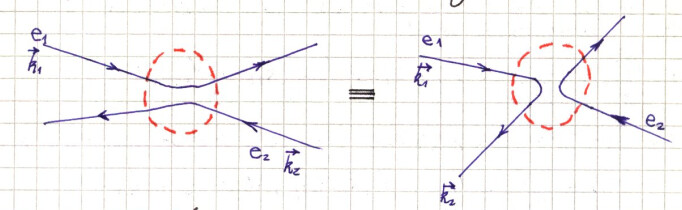
\includegraphics[width=0.65\textwidth]{images/fig_ft2_identical_particles.jpg}

Sean dos estados $\Ket{k'},\Ket{k''}$ con $k^{(i)}$ índice colectivo. 
Si las tengo en una zona común tendré como estado total a $\Ket{k'} \otimes \Ket{k''} $
pero si las partículas son del mismo tipo, 
\[
	\Ket{k'} \otimes \Ket{k''} \qquad \Ket{k''} \otimes \Ket{k'},
\]
representan el mismo sistema cuántico y son ortogonales. No se pueden distinguir estos estados.
\notamargen{No sé si reescribí esta sección diferente a la carpeta porque lo mejoré o si es
equivalente. Se verá en su momento.}

En la zona de interferencia es 
\[
	\Ket{k'}_1 \otimes \Ket{k'}_2 \quad \text{o} \quad \Ket{k''}_1 \otimes \Ket{k''}_2
\]
donde ambos estados son ortogonales y los subíndices numéricos identifican a la partícula. 

\begin{figure}[htb]
	\begin{center}
	\includegraphics[width=0.9\textwidth]{images/teo2_29.pdf}
	\end{center}
	\caption{}
\end{figure} 

	

Entonces un estado general será
\[
	\Ket{K} = c_1 \Ket{k'}_1 \otimes \Ket{k''}_2 + c_2 \Ket{k''}_1 \otimes \Ket{k'}_2
\]
con $|c_1|^2 +|c_2|^2= 1$. 
Esta es la ``degeneración de intercambio'', y la reventaremos con un postulado extra que le
añadiremos a la mecánica cuántica.

Definiremos un operador permutación $P$ que intercambia kets en un producto tensorial.
Es decir que opera según 
\[
	P_{12}( \Ket{k'}_1\otimes \Ket{k''}_2 ) = \Ket{k''}_1\otimes \Ket{k'}_2
\]
y además satisface las siguientes propiedades
\[
	P_{12} = P_{21} \qquad P_{12}^2 = \mathbb{1} \qquad P_{12}^\dagger = P_{12} \qquad 
	P_{12}P_{12}^\dagger = 1 \qquad \text{autovalores:} \; \pm 1
\]

Su función es la de intercambiar etiquetas, no el orden de las partículas.
Sean operadores $\hat{A}_1,\hat{A}_2$ que actúan sobre las partículas 1,2; es decir 
\[
	\hat{A}_1 \equiv \hat{A}_1\otimes\mathbb{1}_2, \qquad 
	\hat{A}_2 \equiv \mathbb{1}_1\otimes\hat{A}_2
\]
Veamos qué sucede sobre autoestados y operadores
\[
	\hat{A}_1 \Ket{a'} \Ket{a''} = a' \Ket{a'} \Ket{a''} \qquad 
	\hat{A}_2 \Ket{a'} \Ket{a''} = a'' \Ket{a'} \Ket{a''} 
\]
\[
	P_{12}A_1P_{12}^{-1}P_{12}\Ket{a'} \Ket{a''} = P_{12} a' \Ket{a'}_1 \Ket{a''}_2 =
	a' \Ket{a''}_1 \Ket{a'}_2
\]
\[
	= P_{12}A_1P_{12}^{-1} \Ket{a''}_1 \Ket{a'}_2 = a' \Ket{a''}_1 \Ket{a'}_2
\]
\[
	= A_2 \Ket{a''}_1 \Ket{a'}_2 = a' \Ket{a''}_1 \Ket{a'}_2
\]
y
\[
	P_{12}\hat{A}_1P_{12}^{-1} = \hat{A}_2, \qquad P_{21} A_1 - A_2 P_{12} = 0
\]
\notamargen{La idea que tenía en la carpeta era la siguiente: si el operador es
simétrico, entonces conmuta con el operador de permutación $P$, no sé si quise
decir eso en las notas de final.}


Luego $\hat{A}$ es simétrico si $[\hat{P}_{12},\hat{A}_{12}]=0$. Sea $[\hat{P}_{12},\hat{H}]=0$ entonces es 
$P_{12}$ constante de movimiento y 
\[
	P_{12} \Ket{\alpha} = \pm \Ket{\alpha}
\]

Un operador que cumple lo de arriba es el hamiltoniano.
Para dos partículas será 
\[
	H = \frac{p_1^2}{2m_1} + \frac{p_2^2}{2m_2} + v(|x_1 - x_2|) + V_e(\vb{x}_1)+ V_e(\vb{x}_2)
\]
donde si las partículas son idénticas se puede hacer $m_1=m_2\equiv m$ y veo que se cumple que
$ [ H, P_{12} ] = 0 $ y $ P_{12} \Ket{\a} = \pm \Ket{\a} $
Defino ahora dos estados, simétrico y antisimétrico
\[
	\Ket{k' k''}_s = \frac{1}{\sqrt{2}}\left( \Ket{k'}_1\Ket{k''}_2 + \Ket{k''}_1\Ket{k'}_2 \right) \qquad 
	\Ket{k' k''}_a = \frac{1}{\sqrt{2}}\left( \Ket{k'}_1\Ket{k''}_2 - \Ket{k''}_1\Ket{k'}_2 \right)
\]
con 
\[
	P_{12}\Ket{\phantom{k}}_s = + \Ket{\phantom{k}}_s \qquad \qquad 
	P_{12}\Ket{\phantom{k}}_a = - \Ket{\phantom{k}}_a
\]
Puedo introducir operadores de simetrización y antisimetrización 
\[
	\hat{S}_{12} \equiv \frac{1}{\sqrt{2}} \left( \mathbb{1} + \hat{P}_{12} \right)
\]
\[
	\hat{A}_{12} \equiv \frac{1}{\sqrt{2}} \left( \mathbb{1} - \hat{P}_{12} \right)
\]
que verifican 
\[
	S^2 = S, \quad  A^2= A, \quad SA=AS=0, \quad [S,A] = 0,
\]
es decir que no son otra cosa que proyectores, 
\[
	\hat{S}_{12} (c_1\Ket{k'}\Ket{k''} + c_2\Ket{k''}\Ket{k'} ) = \frac{1}{\sqrt{2}}(c_1+c_2)
	(\Ket{k'}\Ket{k''} + \Ket{k''}\Ket{k'} )
\]
es simétrico y 
\[
	\hat{A}_{12} (c_1\Ket{k'}\Ket{k''} + c_2\Ket{k''}\Ket{k'} ) = \frac{1}{\sqrt{2}}(c_1-c_2)
	(\Ket{k'}\Ket{k''} - \Ket{k''}\Ket{k'} )
\]
es antisimétrico.
En general se complica bastante con más de dos partículas 
\[
	P_{ij}(\Ket{k'}_1\Ket{k''}_2...\Ket{k^i}_i...\Ket{k^j}_j...) =
	(\Ket{k'}_1\Ket{k''}_2...\Ket{k^j}_i...\Ket{k^i}_j...)
\]
pués tenemos 
\[
	[P_{ij},P_{k\ell}] \neq 0 \quad \text{en general}
\]
Las permutaciones para tres partículas pueden descomponerse en permutaciones de a dos,
como por ejemplo
\[
	P_{123} = P_{12}P_{13} 
\]
\[
	P_{123}\Ket{k'}\Ket{k''}\Ket{k'''} = P_{12}\Ket{k'''}\Ket{k''}\Ket{k'} = \Ket{k''}\Ket{k'''}\Ket{k'}
\]

Con tres partículas hay $3!$ estados; uno totalmente simétrico $\Ket{\phantom{k}}_s$, uno totalmente antisimétrico 
$\Ket{\phantom{k}}_a$ y cuatro sin simetría definida.
Los estados con simetría definida serán 
\begin{align*}
	\Ket{k'k''k'''}_{s/a} = \frac{1}{\sqrt{6}}&\left( \Ket{k'k''k'''} +  \Ket{k''k'''k'} + \Ket{k'''k'k''}\right. \\
	& \left. \pm \Ket{k''k'k'''} \pm \Ket{k'k'''k''} \pm \Ket{k'''k''k'} \right)
\end{align*}
donde el $\Ket{}_a$ tiene el signo $(-)$ en las permutaciones anticíclicas y el $(+)$ en las cíclicas.
Existe un determinante de Slater como método mnemotécnico de obtener los estados $\Ket{}_a$.
\[
	\Ket{ \Psi }_a = \frac{1}{3!}\begin{vmatrix} \; \Ket{k'} & \Ket{k''} & \Ket{k'''} \\  
	\; \Ket{k'} & \Ket{k''} & \Ket{k'''} \\ \; \Ket{k'} & \Ket{k''} & \Ket{k'''} \end{vmatrix}
\]
La obtención de estos estados corresponde a aplicar 
\[
	A_{123} = \frac{1}{\sqrt{3!}}\left( \mathbb{1} + P_{231} + P_{312} - P_{212} - P_{132} - P_{321} \right)
\]
\[
	( \mathbb{1} + P_{23}P_{21} + P_{31}P_{32} - P_{21}P_{23} - P_{13}P_{12} - P_{32}P_{31} )
\]
Si dos $k^{(i)}$ coinciden ya no hay estado antisimétrico posible.

\section{Postulado de simetrización}

Permitirá romper la degeneración de intercambio. 
Postulamos que toda partícula es de uno de dos tipos de acuerdo a su simetría 

\begin{center}
\begin{tabular}{|c|l|l|l|l|}
\multirow{2}{*}{Sistemas de N part. idénticas} & N & simetrica & BE & entero\\
& N & antisimetrica & FD & semientero
\end{tabular}
\end{center}

\begin{center}
\begin{tabular}{lll}
Función de onda & Estadística & Spin \\
\hline \\
Simétrica & Bosones $P_{ij}\Ket{ N \text{ bosones}} = 
+ \Ket{ N \text{ bosones}} $ & Entero\\
Antisimétrica & Fermiones $P_{ij}\Ket{ N \text{ fermiones}} = 
- \Ket{ N \text{ fermiones}} $ & Semi-entero
\end{tabular}
\end{center}

En la naturaleza no ocurren simetrías mixtas.

% \subsection{Principio de exclusión de Pauli}

Para fermiones, suponiendo un sistema de dos partículas idénticas, es
\[
	\Ket{ \Psi }_a = \frac{1}{\sqrt{2}}( \Ket{k'}_1\Ket{k''}_2 - \Ket{k''}_1\Ket{k'}_2)
\]
y entonces si $k'=k''$ se tiene que 
\[
	\Ket{ \Psi }_a = 0.
\]
de manera que no es posible tener dos fermiones con iguales números cuánticos.
Esto es el principio de exclusión de Pauli. 
Por el contrario los bosones sí pueden tener iguales números cuánticos.

\notamargen{En la carpeta hay un ejemplo que no entiendo en la p81 donde la moraleja
es que el hamiltoniano no tiene modo de vincular estados de bosones con estados de
fermiones. Habría que ver de entenderlo y juzgar luego si aporta introducirlo aquí.}


\subsection{Sistema de dos electrones de spin $1/2$}

Sistema de dos electrones de spin $1/2$, que son fermiones. Sea que el hamiltoniano
no depende del spin total y por ello $[H,S]=0$  con $S = S_1 + S_2$. Se tendrá 
\[
	\Ket{\Psi}^{sist} = \Ket{\Psi}^{spa} \otimes \Ket{\Psi}^{spin},
\]
pero como $\Ket{\Psi}^{sist}$ tiene que ser antisimétrica tendremos 
\[
	P_{12} \Ket{\Psi}^{sist} = - \Ket{\Psi}^{sist} 
\]
que, según la separación anterior, implica que 
\[
	P_{12} \Ket{\Psi}^{sist} = P_{12} \Ket{\Psi}^{spa} \otimes P_{12}\Ket{\Psi}^{spin} 
\]

No obstante, aún antes de saber lo de la parte espacial ya tengo información de la
parte de spin.
Para dos electrones con spin $1/2$ se tiene $j_1+j_2$ entonces $ 0 \leq j \leq 1 $ de modo que $|m_1|\leq j_1$ y
$|m_2|\leq j_2$ entonces $0 \leq S \leq 1$ y $|m_{s_1}|\leq s_1$ y $|m_{s_2}|\leq s_1$.
\[
	\left.\begin{aligned}
	& \Ket{\uparrow \uparrow} \\
	& \Ket{\downarrow \downarrow } \\
	& \frac{1}{\sqrt{2}}( \Ket{ \uparrow\downarrow }+\Ket{ \downarrow\uparrow} )
	\end{aligned}
	\right\} \; \text{triplete} \; s=1 \qquad \text{Estados simétricos}
\]
\[
	\left.\begin{aligned}
	\frac{1}{\sqrt{2}}( \Ket{\uparrow\downarrow} - \Ket{\downarrow\uparrow} )
	\end{aligned}
	\right\} \; \text{singlete} \; s=0 \qquad \text{Estados antisimétricos}
\]

Además se tiene $ [P_{12}, S_\pm] = 0 $ y obtengo los del triplete con la bajada y subida $S_\pm$,
de modo que todos están relacionados.
Luego, $ P_{12} \ket{\Psi}^{spin} $ será simétrico $S=1$ o antisimétrico $S=0$ y esto es 
independiente del hamiltoniano $H$ y viene de que pudimos separar parte espacial y spin.

Ahora bien, como simétrico por antisimétrico en $S\otimes A$ es antisimétrico
\[
	P_{12} \Ket{\Psi}_{sist} =
	P_{12}^{spa} \Ket{\Psi}_{spa} \otimes P_{12}^{spi} \Ket{\Psi}_{spin}
\]
y se tienen en cada caso $A \otimes S$ en $S=1$ o bien $S \otimes A$ en $S=0$ será
en el primer caso $\Ket{\Psi}_{spa}$ antisimétrica con $(-1)^\ell$ y $\ell$ impar 
y en el segundo caso $\Ket{\Psi}_{spa}$ simétrica con $(-1)^\ell$ y $\ell$ par. 


Entonces
\begin{gather*}
	\begin{aligned}
	s=0 \qquad \Rightarrow \; &\Ket{\Psi}^{spa} \text{es simétrica} \\
	s=1 \qquad \Rightarrow \; &\Ket{\Psi}^{spa} \text{es antisimétrica}
	\end{aligned}	
\end{gather*}	

Vistos desde el centro de masa dos electrones verifican que $ P_{12} = \Pi $ 
(el operador $P_{12}$ es paridad) y entonces
\notamargen{Dos electrones solo pueden acoplarse a impulso total par $\vb J = \vb L + \vb S$.
Acá hay un mix de explicaciones, evidentemente carpeta no coincidía con las notas.}
\[
	P_{12}\Ket{n\ell m} = (-1)^\ell \Ket{n\ell m}
\]
\[
	\ell \;\text{par} \; \rightarrow \Ket{\Psi}^{spa} = P_{12} \Ket{\Psi}^{spa} \qquad 
	\ell \;\text{impar} \; \rightarrow -\Ket{\Psi}^{spa} = P_{12} \Ket{\Psi}^{spa}
\]
Necesitaré $\ell$ par con $s=0$ entonces $\ell+s=j$ par. En cambio, si $\ell$ impar con $s=1$ entonces 
$\ell+s=j$ par. Dos electrones sólo se acoplan a momento total $j$ par.

Podemos poner los siguientes estados 
\[
	\Ket{ \Psi }_{sa} = \frac{1}{\sqrt{2}}( \Ket{k'}\Ket{k''} \pm \Ket{k''}\Ket{k'})
\]

Teniendo una relación $A\Ket{a_i} = a_i \Ket{a_i}$ para un operador $A$, 
un autoestado con una partícula con autovalor $a_1$ y otra con $a_2$ se escribe
\[
	\Ket{ \Psi_F }_{sa} = \frac{1}{\sqrt{2}}( \Ket{a'}\Ket{a''} \pm \Ket{a''}\Ket{a'}),
\]
donde habrá que simetrizar o antisimetrizar si las partículas son bosones o fermiones,
respectivamente. Usando $ \text{Prob}_{(a_1,a_2)} = | _{S/A}\Braket{\Psi_f|\Psi}_{S/A} |^2 $,
la probabilidad será
\begin{multline*}
	\text{Prob}\; = |_{sa}\Braket{\Psi|\Psi}_{sa}|^2 =  \\
	\left|\frac{1}{2}(_1\Bra{a'}_2\Bra{a''} \pm _1\Bra{a''}_2\Bra{a'})(\Ket{k'}_1\Ket{k''}_2 \pm 
	\Ket{k''}_1\Ket{k'}_2)\right|^2 =
\end{multline*}
\begin{multline*}
 	= \frac{1}{4}\left| \Bra{a'}\Bra{a''}\Ket{k'}\Ket{k''} \pm \Bra{a''}\Bra{a'}\Ket{k'}\Ket{k''} 
	\right. \pm \\
	\left. \Bra{a'}\Bra{a''}\Ket{k''}\Ket{k'} \pm \Bra{a''}\Bra{a'}\Ket{k''}_1\Ket{k'} \right|^2 \\
	= \frac{1}{4}\left| 2\Braket{a'|k'}\Braket{a''|k''} \pm 2\Braket{a''|k'}\Braket{a'|k''}\right|^2, 
\end{multline*}
que se puede escribir como
\[
	\text{Prob}\; = \left| \underbrace{\Braket{a'|k'}\Braket{a''|k''}}_{\text{término directo}} \pm 
	\underbrace{\Braket{a''|k'}\Braket{a'|k''}}_\text{término de intercambio}\right|^2
\]
donde hemos marcado un término directo y uno de intercambio, asociado con la probabilidad de que una
partícula pase al estado de la otra. El signo $+$ es para bosón y el signo $-$ para fermión. El término 
directo asocia entonces $k_1 \to a_1$ y $k_2 \to a_2$ mientras que el de intercambio $k_1 \to a_2$ y 
$k_2 \to a_1$.

Al explicitar la cuenta con el módulo al cuadrado obtenemos la interferencia (de sentido cuántico) que
aparece porque son indistinguibles las partículas
\begin{multline*}
	\text{Prob}\; = |_{sa}\Braket{\Psi|\Psi}_{sa}|^2 = \left| \Braket{a'|k'}\Braket{a''|k''} \right|^2 + 
	\left|\Braket{a''|k'}\Braket{a'|k''}\right|^2  \\
	\pm 2\mathcal{Re}\left(\underbrace{ \Braket{a'|k'}\Braket{a'|k''}^*\Braket{a''|k''}\Braket{a''|k'}^* 
	}_\text{Interferencia}\right)
\end{multline*}

Vemos que aparece una interferencia que será importante solamente si hay solapamiento. En el caso de no 
solaparse o con partículas clásicas sólo el primer término es de importancia.

Esto puede aplicarse al caso ilustrativo de la ``teleportación''.
Consideremos el ejemplo de medición de electrones en lugares apartados, como

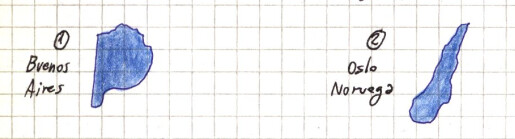
\includegraphics[width=0.6\textwidth]{images/fig_ft2_extra_identical.jpg}

En Buenos Aires tenemos $\psi_1 = \Braket{\vbx | k_1} \neq 0 $ y $\psi_2 = \Braket{\vbx | k_2} = 0 $
mientras que en Oslo $\psi_1 = 0 $ y $\psi_2 \neq 0 $ lo que significa que el electrón de Oslo en $\psi_2$
no lo puedo hallar en Buenos Aires.
Luego, $\Braket{\vbx|a_1}\neq 0 $ y $\Braket{\vbx|a_2} = 0 $ siendo la primera la variable dinámica asociada
al detector en Buenos Aires.


\section{El átomo de helio}

Posee dos protones, dos neutrones y dos electrones. La figura bajo estas líneas ilustra el sistema
coordenado

\includegraphics[width=0.4\textwidth]{images/teo2_30.pdf}

El hamiltoniano se puede escribir 
\[
	H = \frac{p_1}{2m} + \frac{p_2}{2m} - \frac{2e^2}{r_1} -  \frac{2e^2}{r_2} + \frac{e^2}{r_{12}}
\]
y si el último término es $\sim 0$ decimos que en ese caso $H$ está desacoplado y tenemos una
función de onda del tipo
\[
	\Psi = \Psi_1 \otimes \Psi_2.
\]
Dado que se verifica
\[
	[\vb{H},\vb{S}] = 0 
	\qquad 
	\vb{S} = \vb{S}_1 + \vb{S}_2 = 
	\begin{cases} 
	0 \\ 
	1 
	\end{cases}
\]
se da que $S$ es constante de movimiento y para la $\Ket{\psi_{spin}}$ se tiene 
\[
	S=0 \qquad \frac{1}{\sqrt{2}}( \Ket{ \uparrow\downarrow }-\Ket{ \downarrow\uparrow}) \quad \text{singlete}
\]
\[
	S=1 \qquad \begin{aligned}
	& \Ket{\uparrow \uparrow} \\
	& \Ket{\downarrow \downarrow } \\
	& \frac{1}{\sqrt{2}}( \Ket{ \uparrow\downarrow }+\Ket{ \downarrow\uparrow} )
	\end{aligned} \quad \text{triplete}
\]
Sea un electrón  en el estado fundamental $ \Ket{100}$ y otro en algún estado excitado $ \Ket{n\ell m}$,
se tendrán
\[
	\Ket{\Psi}_{He} = \frac{1}{\sqrt{2}}\left(  \Ket{100}\Ket{n\ell m} \pm  \Ket{n\ell m}\Ket{100}
	\right) \Ket{\Psi_{spin}}
\]
donde el signo $+$ es para $S=0$ y el signo $-$ para $S=1$ y vemos que $\Ket{\Psi_{spin}}$ tiene simetría
bien definida.
Así, con $S=0$, será
\[
	\Ket{\Psi}_{He} = \frac{1}{\sqrt{2}}\left( \Ket{100}\Ket{n\ell m} + \Ket{n\ell m}\Ket{100}\right) 
	\frac{1}{\sqrt{2}}( \Ket{ \uparrow\downarrow }-\Ket{ \downarrow\uparrow})
\]
y en cambio con $S=1$
\[
	\Ket{\Psi}_{He} = \frac{1}{\sqrt{2}}\left(  \Ket{100}\Ket{n\ell m} - \Ket{n\ell m}\Ket{100}\right) 
			\begin{cases}
	                   \Ket{\uparrow \uparrow} \\
			   \Ket{\downarrow \downarrow } \\
			   \frac{1}{\sqrt{2}}( \Ket{ \uparrow\downarrow }+\Ket{ \downarrow\uparrow} )
	                  \end{cases} .
\]
\notamargen{Lo que uno simetriza o antisimetriza son las partículas idénticas.}

Ahora introduzcamos la interacción con el término $e^2/r_{12}$. Consideremos, en teoria de perturbaciones,
que 
\[
	E_{He} = E_{100} + E_{n\ell m} + \Delta E
\]
donde 
\[
	\Delta E = \Braket{\Psi|\frac{e}{r_{12}}|\Psi}
\]
y el término en el {\it sandwich} lo considero una perturbación.
Haciendo la cuenta explícitamente
\begin{multline*}
	\Delta E = \Bra{\Psi^{spin}}^\dagger \frac{1}{2}\left(\Bra{100}\Bra{n\ell m} \pm \Bra{n\ell m}\Bra{100}
	\right) \frac{e}{r_{12}} \times \\
	\left(\Ket{100}\Ket{n\ell m} \pm \Ket{n\ell m}\Ket{100}\right)\Ket{\Psi^{spin}}
\end{multline*}
\[
	\Delta E = \Bra{100}\Bra{n\ell m}\frac{e}{r_{12}}\Ket{100}\Ket{n\ell m} \pm  
	\Bra{n\ell m}\Bra{100}\frac{e}{r_{12}}\Ket{100}\Ket{n\ell m}
\]
donde vemos que el operador es invariante antes $1 \to 2, 2 \to 1$ pués $|\vbx_1 - \vbx_2| = |\vbx_2 - \vbx_1| 
\equiv r_{12}$ y que escribiremos más resumidamente como
\[
	\Delta E = I \pm J.
\]

Para calcular necesitaremos integrar metiendo una identidad
\[
	\int d^2x_1 d^2x_2 \: \Bra{100}\Bra{n\ell m}\frac{e}{r_{12}} \left[ 
	\Ket{x_1}\Ket{x_2} \Bra{x_1}\Bra{x_2}
	\right] \Ket{100}\Ket{n\ell m}
\]
tras lo cual, luego de un amasaje veríamos que
\[
	I = \int d^2x_1 d^2x_2 \: \frac{e}{r_{12}} \:
	|\Psi_{100}(x_1)|^2 |\Psi_{n\ell m}(x_2)|^2
\]
\[
	J = \int d^2x_1 d^2x_2 \: \frac{e}{r_{12}} \: 
	\Psi_{100}(x_1) \Psi_{n\ell m}(x_2) \Psi_{100}(x_2)^* \Psi_{n\ell m}(x_1)^*
\]

En un diagrama ilustrativo sería algo como

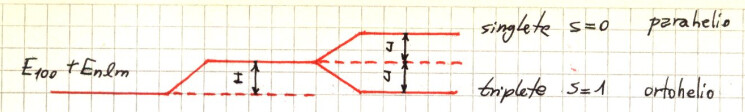
\includegraphics[width=0.8\textwidth]{images/fig_ft2_extra_identical2.jpg}

\begin{figure}[htb]
	\begin{center}
	\includegraphics[width=1.0\textwidth]{images/teo2_15.pdf}
	\end{center}
	\caption{}
\end{figure} 

Vemos un efecto debido al spin de las partículas que no está en el hamiltoniano (puesto que
el $H$ no depende del $\vb S$).
Esta separación de los niveles en $\pm J$ se debe al carácter de fermión de las partículas.
Es una consecuencia de la simetría de la función de onda.



\begin{ejemplo}{\bf Ejercicio 1}

Para la parte a) considera el conjunto $ \{ \Ket{0,-}, \Ket{0,+}, \Ket{1,-}, \Ket{1,+}, ... \} $
que son los $N$ primeros.
Entonces
\[
	E = \sum_{n=0}^{[N/2]-1} \: 2 \hbar \omega \left( n + \frac 1 2 \right) + 
	\hbar \omega \left( \left[ \frac{n}{2} \right] + \frac 1 2 \right)_{\text{ N impar }}
\]

Para la parte b) considero $N=2$ y $ \Ket{0,-} \otimes \Ket{0,+} $ y para ser la función de onda
necesitaré que sea antisimétrica porque son fermiones.
Entonces
\[
	\Ket{\Psi} = \frac{1}{\sqrt{2}}( \Ket{0,-} \otimes \Ket{0,+} - \Ket{0,+} \otimes \Ket{0,-} )
\]
y
\[
	A_{12} ( \Ket{0,-} \otimes \Ket{0,+} ) = \Ket{\Psi}
\]

El hamiltoniano será
\[
	H = \frac{p_1^2}{2m} + \frac{p_2^2}{2m} + \frac{1}{2} m \omega^2 x_1^2
	+  \frac{1}{2} m \omega^2 x_2^2
\]
y entonces
\[
	\Braket{\Psi|H|\Psi} = \frac{1}{2}
	\left( 
	\Bra{0,-} \otimes \Bra{0,+} - \Bra{0,+} \otimes \Bra{0,-}
	\right) H \left( 
	\Ket{0,-} \otimes \Ket{0,+} - \Ket{0,+} \otimes \Ket{0,-}
	\right),
\]
pero com el $H$ no toca los spines entonces serán nulos el primero y el cuarto. Luego
\[
	\Braket{\Psi|H|\Psi} = \frac{1}{2}
	\left(
	\Bra{0,-} \Bra{0,+} H \Ket{0,-}\Ket{0,+} + 
	\Bra{0,+} \Bra{0,-} H \Ket{0,+} \Ket{0,-}
	\right)
\]
y como el $H=H_1+H_2$ cuentas más o menos {\it straighforward} llevan a 
\[
	\Braket{\Psi|H|\Psi} = \hbar \omega.
\]
\notamargen{En la carpeta hay una recarga extra sobre la notación de indicar con un 1 o 2 si
es la primer o segunda partícula; creo que es innecesario, sabemos que el orden de los ket y bra
en esta escritura {\it matters}.}

Ahora queremos calcular el $J^2$ para ello escribamos el estado según
\[
	\Ket{\Psi} = \frac{1}{\sqrt{2}}
	\left( 
	\Ket{0}_1 \otimes \Ket{-}_1 \otimes \Ket{0}_2 \otimes \Ket{+}_2 -
	\Ket{0}_1 \otimes \Ket{+}_1 \otimes \Ket{0}_2 \otimes \Ket{-}_2
	\right)
\]
y reacomodando un poco,
\[
	\Ket{\Psi} = \frac{1}{\sqrt{2}}
	\left( 
	\Ket{0}_1 \otimes \Ket{0}_2 \otimes 
	\left[ \Ket{-}_1  \Ket{+}_2 - \Ket{+}_1 \Ket{-}_2 \right] \right)
\]
y el spin total es nulo, entonces no tenemos dirección privilegiada.
 
\end{ejemplo}

\begin{ejemplo}{\bf Ejercicio 2}

Son dos partículas de spin $3/2$. Por teoría de suma de momentos angulares popdría tener
$3,2,1,0$

\[
	\Ket{j, m} = \sum_{m_1,m_2} \: \Ket{j_1,j_2,m_1,m_2} \Braket{j_1,j_2,m_1,m_2|j,m}
\]
y cuando le aplicamos la permutación
\begin{multline*}
	P_{12} \Ket{j, m} = \sum_{m_1,m_2} \: \Ket{j_2,j_1,m_2,m_1} \Braket{j_1,j_2,m_1,m_2|j,m} = \\
	\sum_{m_1,m_2} \: \Ket{j_1,j_2,m_1,m_2} \Braket{j_1,j_2,m_2,m_1|j,m}
\end{multline*}
vemos que el coeficientes no cambia pero que, puedo sin pérdida de generalidad intercambiar las
letras (son mudas).

Para que sea una función de ferminiones válida necesitaré
\[
	\Braket{j_1,j_2,m_2,m_1|j,m} = - \Braket{j_1,j_2,m_1,m_2|j,m} = (-1)^{j_1+j_2-J} \Braket{}
\]
donde lo último viene de propiedades de los coeficientes.
Luego será $(-1)^{j_1+j_2-J} = -1$ y $3-J$ es natural par.
La simetrización implicará que se acople solamente a spin 2 y spin 0.

\end{ejemplo}

\begin{ejemplo}{\bf Ejercicio 3}
 
Es similar a este. 
 
\end{ejemplo}

\begin{ejemplo}{\bf Ejercicio 4}
 
Misma cuenta, pero para bosones. Llegaremos a $\ell_1 + \ell_2 - L $  para $N$ pares y $2\ell - L$
para $N$ impares.
 
\end{ejemplo}

\begin{ejemplo}{\bf Ejercicio 5}

Vemos solamente la parte b). La base en la cual estamos trabajando es
\[
	\{  \Ket{-1,-1,-1}, \Ket{-1,-1,0}, \Ket{-1,-1,1}, ..., \Ket{1,1,1} \}
\]
y tiene dimensión 27. Estos componentes serán simétricos frente al intercambio de dos partículas.
Por ejemplo para $\Ket{-1,-1,-1}, \Ket{0,0,0}, \Ket{1,1,1}$ es
\[
	\frac{1}{\sqrt{3}} \left( \Ket{-1,-1,0} + \Ket{-1,0,-1} + \Ket{0,-1,-1}  \right)
\]
donde los últimos dos los incluyo para que al intercambiar 1,2 no se altere nada y lo mismo al
intercambiar 2,3.
En general, para los estados que tienen dos repetidos será
\[
	\frac{1}{\sqrt{3}} \left( \Ket{b,b,b} + \Ket{b,a,b} + \Ket{a,b,b}  \right)
\]
que para $a=-1,0,1, b=-1,0,1$ con $a\neq b$ serán seis estados.

Ahora restará cubrir los estados que tienen los tres números distintos, 
\[
	\frac{1}{\sqrt{6}} \left( 
	\Ket{-1,0,1} + \Ket{0,-1,1} + \Ket{1,0,-1} +
	\Ket{1,-1,0} + \Ket{0,1,-1} + \Ket{-1,1,0}
	\right)
\]
y vemos que hay que sumar todos los estaods que tienen una vez cada número.
Ahora tendremos en total $1+3+6$ estados que son simétricos. Los restantes 17 son o bien
antisimétricos o sin simetría definida.


\end{ejemplo}

% \bibliographystyle{CBFT-apa-good}	% (uses file "apa-good.bst")
% \bibliography{CBFT.Referencias} % La base de datos bibliográfica

\end{document}
